 \documentclass[12pt]{article}

\usepackage[T2A]{fontenc}
\usepackage[utf8]{inputenc}
\usepackage[russian]{babel}
\usepackage{amsmath,amssymb,amsfonts,amsthm}
\usepackage{indentfirst}
\usepackage{titlesec}
\usepackage{setspace}
\usepackage{graphicx}

\renewcommand{\topfraction}{1.0}
\renewcommand{\bottomfraction}{1.0}
\renewcommand{\textfraction}{0.0}

\usepackage{epstopdf}
\epstopdfsetup{suffix=}

\usepackage{tikz}

\usepackage{caption}
  \captionsetup[figure]{labelsep=period,name=Рис.}

\titleformat*{\section}{\Large\bfseries\filcenter}
\titleformat*{\subsection}{\large\bfseries\filcenter}
\titleformat*{\subsubsection}{\normalsize\bfseries\filcenter}

\usepackage{cmap}                   % поиск в PDF

\usepackage{geometry}
    \geometry{a4paper}
    \geometry{top=20mm}
    \geometry{bottom=20mm}
    \geometry{left=30mm}
    \geometry{right=15mm}  

\usepackage{enumitem}  

\theoremstyle{plain}
\newtheorem{definition}{Определение}    


\graphicspath{{./Картинки для презентации/}}
    
 
%======================================================================
%======================================================================


\begin{document}

\thispagestyle{empty} % нумерация выкл.

\section*{\centerline{РЕФЕРАТ}}

{\raggedright

\noindent
Михайлов А. В. РАЗРАБОТКА ПРОЦЕДУРЫ ПРОГНОЗИРОВАНИЯ ПРОМЕЖУТКА ВАРИАЦИИ МОМЕНТА ПРИБЫТИЯ ВОЗДУШНОГО СУДНА, выпускная квалификационная работа: стр.~\pageref{lastpage}, рис.~8, библ.~9~назв.

}

\medskip

{\raggedright

\noindent
Ключевые слова: УПРАВЛЕНИЕ ВОЗДУШНЫМ ДВИЖЕНИЕМ, ВОЗДУШНЫЕ ТРАССЫ, СХЕМЫ ЗАДЕРЖКИ, ПОТОКИ ВОЗДУШНЫХ СУДОВ, АЛГОРИТМЫ БЕСКОНФЛИКТНОГО СЛИЯНИЯ, ПРОГНОЗИРОВАНИЕ МОМЕНТА ПРИБЫТИЯ.

}

\medskip

\noindent
Целью работы является разработка и реализация алгоритма прогнозирования прибытия воздушного судна (ВС) в контрольные точки его движения по трассе. Входной информацией для алгоритма служит топографическая конфигурация системы воздушных трасс в том или ином районе управления воздушным движением (УВД). Такая конфигурация включает в себя описание контрольных точек трасс (координаты и допустимый диапазон скоростей ВС в точке), схемы их соединения (порядок прохода ВС по этим точкам), наличие вариантов трасс и схем задержек (которые подразумевают для некоторой контрольной точки несколько возможных следующих точек), участков возможного спрямления движения. В результате работы алгоритма для каждой точки каждой трассы вычисляется множество моментов возможного прибытия ВС в эту точку (в предположении что в начальный момент времени ВС вошло на контроль на первую точку своей трассы). Такая информация необходима для работы алгоритмов безопасного слияния потоков ВС в точках соединения их трасс, например, в аэропортовой зоне, куда приходят несколько потоков ВС с различных направлений. Создан формат представления воздушных трасс. Разработанный алгоритм реализован в виде программы на языке C++.


\newpage
%====================================================

\setcounter{page}{2}

\setstretch{1.3}

\tableofcontents

\newpage


%=======================================================================
\section*{Введение}
\addcontentsline{toc}{section}{Введение}

\begin{figure}[p]
  \centering

  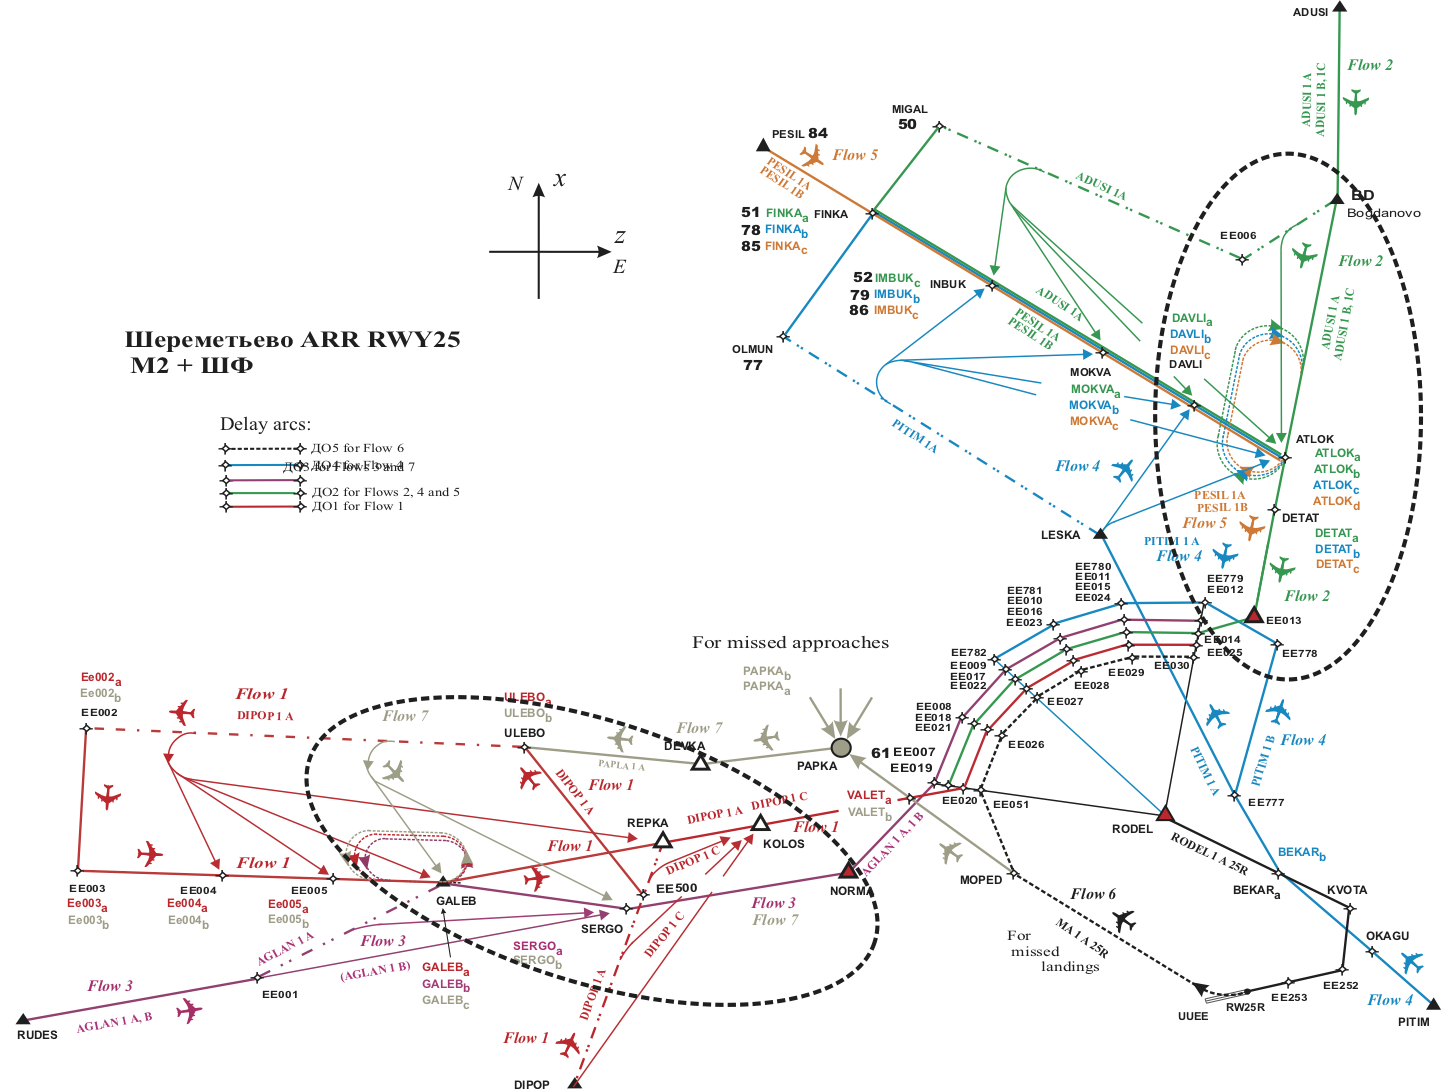
\includegraphics[height=0.99\textwidth,angle=90]{Complete.png}

  \caption{Схема части воздушных трасс в аэропортовой зоне а/п Шереметьево}
  \label{fig:Sherem}
\end{figure}

В настоящее время движение воздушных судов (ВС) происходит по воздушным трассам, состоящим из коридоров в горизонтальной плоскости и эшелонов в вертикальной. При этом трассы могут разветвляться или соединяться (рис.~\ref{fig:Sherem}). В точке соединения трасс возникает задача слияния потоков самолётов в единую посадочную очередь. Такая задача особенно актуальна в зонах подхода и зонах аэродромов, где плотность воздушного движения высока. Основным требованием при слиянии потоков ВС является наличие минимального безопасного временного интервала между моментами прибытия судов в точку слияния.

Поэтому имеется ряд задач:
\begin{enumerate}[topsep=-0.5\parsep,itemsep=-0.5\parsep]
  \item на основе топографического описания воздушных трасс спрогнозировать возможные моменты прибытия ВС в контрольные точки его трассы;

  \item на основе этой информации, а также с использованием номинального расписания прибытия ВС, разрабатывается фактическое расписание прибытия ВС, обеспечивающее безопасность в точках слияния потоков ВС;

  \item на основе построенного расписания и топографического описания воздушных трасс вырабатываются рекомендации диспетчерам управления воздушным движением (УВД) по регулированию движения каждого планируемого ВС для выдерживания им режима движения, требуемого для прибытия в контрольные точки в требуемые моменты времени.
\end{enumerate}

В рамках данной работы предлагается алгоритм решения первой из этих задач, то есть построение множеств возможных моментов прибытия ВС в те или иные контрольные точки его воздушной трассы, которые могут быть реализованы с использованием задержек и ускорений, связанных с вариацией скорости движения ВС, задержек, обеспечиваемых схемами задержки, ускорениями, обеспечиваемыми участками спрямления движения. 

\section{Постановка задачи}

В рамках работы были поставлены следующие задачи:
\begin{enumerate}[topsep=-0.5\parsep,itemsep=-0.5\parsep]
  \item изучить типовые элементы воздушных трасс и схем задержек; 
  \item придумать формальное описание этих элементов;
  \item предложить формат представления данных о воздушной трассе в файле;
  \item разработать структуры для хранения этих данных в памяти компьютера;
  \item создать процедуры чтения этих данных из файла;
  \item разработать математическую модель движения ВС по тем или иным элементам воздушной трассы;
  \item разработать процедуру, использующую модель движения ВС и структуру воздушной трассы, для формирования множества возможных моментов прибытия ВС в контрольные точки трассы.
\end{enumerate}

\section{Типовые элементы воздушных трасс и схем задержек}

При рассмотрении схемы трасс, приведенной на рис.~\ref{fig:Sherem}, можно выделить следующие типовые элементы трассы.

\textbf{1. Линейный участок трассы}, включающий две или более контрольных точек, по которым ВС движется последовательно.

\textbf{2. Стандартная схема задержки} (рис.~\ref{fig:StandardScheme}). На стандартной схеме задержки ВС сходит с трассы, разворачиваясь на $180^\circ$, некоторое время движется в обратном направлении, после чего снова разворачивается и идёт по той же трассе или параллельно ей на более низком эшелоне. 

\begin{figure}[h]
  \centering

  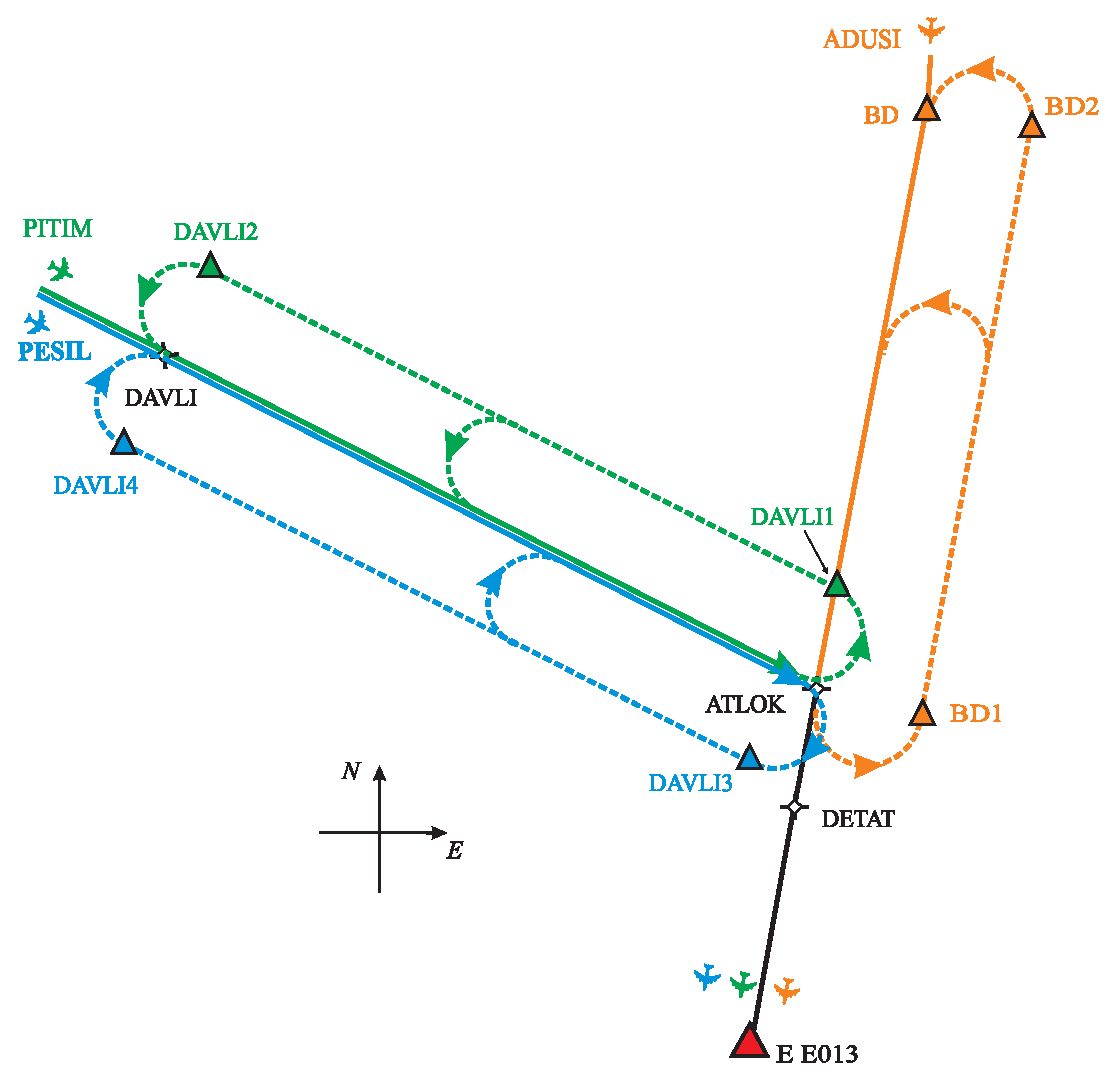
\includegraphics[width=11cm]{Scheme01_plane.eps}    %Рис1

  \caption{Стандартная схема задержки} 
  \label{fig:StandardScheme}
\end{figure}

Стандартная схема характеризуется тремя точками:
\begin{enumerate}[topsep=-0.5\parsep,itemsep=-0.5\parsep]
  \item точкой начала обратного разворота; 
  \item точкой конца дуги разворота;
  \item предельной точкой возможного обратного движения;
\end{enumerate}
Четвертая точки, точка конца дуги разворота, возвращающего на трассу, подразумевается.  Важно отметить, что ВС может сделать разворот, возвращающий на трассу в любой точке прямолинейного отрезка 2--3 обратного движения и выйти на соответствующую точку отрезка~4--1. Четвертая точка не включается в о писание схемы, хотя и отмечена в схемах на рис~\ref{fig:StandardScheme}, поскольку в вычислениях неважно, на какую именно точку вернулось ВС. Время повторного движения в прямом направлении считается равным времени обратного движения.


\textbf{3. Схема задержки веерного типа} (рис.~\ref{fig:VeerScheme}. На схеме задержки веерного типа ВС выполняет поворот, уходя с маршрута движения, и двигается по дуге окружности с центром в следующем контрольном пункте, сходя с этой дуги на точку слияния при достижении нужной задержки. 

\begin{figure}[h]
  \centering

  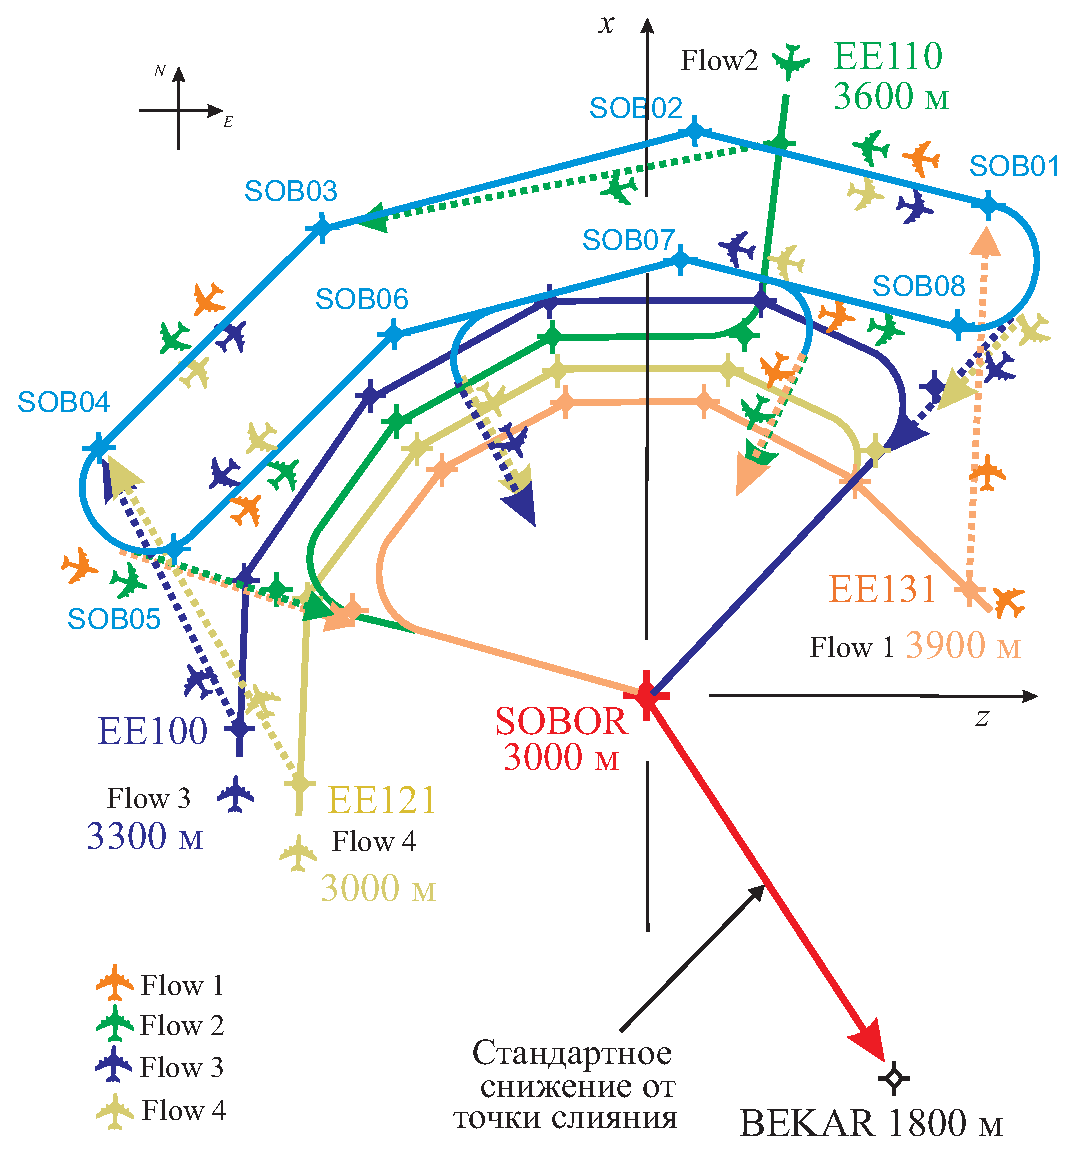
\includegraphics[width=11cm]{Scheme02_plane.eps}    %Рис2

  \caption{Схема задержки веерного типа} 
  \label{fig:VeerScheme}
\end{figure}

Веерная схема характеризуется точкой слияния, а также точками, расположенными на дуге ожидания. Сход на точку слияния возможен с любой точки отрезков, соединяющих точки, расположенные на дуге ожидания.

\textbf{4. <<Тромбон>>} (рис.~\ref{fig:TromboneScheme}). Эта схема является объединением веерной схемы и стандартной схемы задержки. Данная схема состоит из стандартной схемы задержки, развёрнутой под углом к основному маршруту движения. При необходимости выполнения задержки ВС сходит с основного маршрута движения на данную схему, продолжает движение на том же эшелоне, удаляясь от основного маршрута движения. Затем, при необходимости выполнения длительной задержки, выполняет разворот на $180^\circ$ со снижением и продолжает движение к основному маршруту движения. Выработав необходимую задержку, ВС выполняет сход (разворот) со снижением с плеча тромбона в точку слияния. 

\begin{figure}[h]
\centering

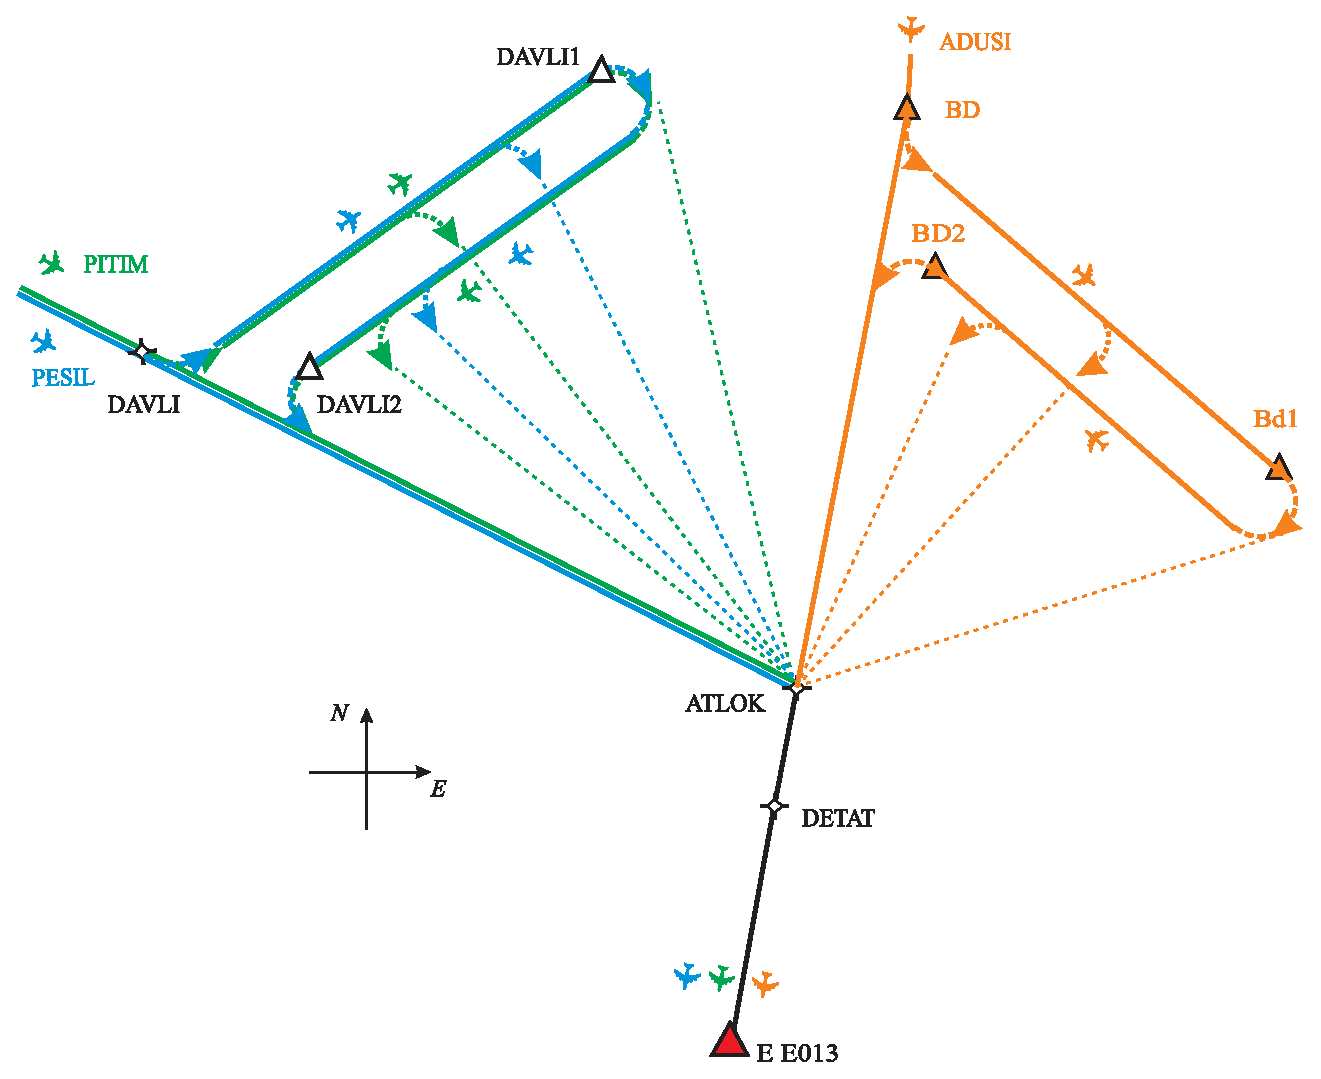
\includegraphics[width=11cm]{Scheme03_plane.eps}    %Рис3

\caption{Схема задержки типа <<тромбон>>} 
\label{fig:TromboneScheme}
\end{figure}

Соответственно, <<тромбон>> задаётся 
\begin{enumerate}[topsep=-0.5\parsep,itemsep=-0.5\parsep]
  \item точкой схода на боковое плечо; 
  \item точкой конца бокового плеча и начала обратного разворота;
  \item точкой окончания обратного движения к трассе;
  \item точкой нацеливания при сходе с <<тромбона>>, которая также является и точкой трассы, по которой ВС идет в случае отсутствия задержки.
\end{enumerate}

\medskip

\textbf{5. Участок спрямления} (рис.~\ref{fig:Sherem}, красная трасса на точках DIPOP--EE500--REPAK--KOLOS). Участок спрямления в каком-то смысле является схемой ускорения, обратной веерной схеме задержки. Если в веерной схеме нормальным является прохождение мимо схемы без схода на дугу ожидания, то на участке спрямления нормальным является движение по всем точкам трассы с возможным сходом на конечную точку при необходимости. Соответственно, с точки зрения своего описания участок спрямления полностью эквивалентен веерной схемы задержки.

\medskip

Таким образом, можно видеть, что имеется три основных элемента, из которых формируются воздушные трассы: линейный участок движения, участок спрямления и стандартная схема задержки. Особенностью третьей схемы является то, что при возврате на трассу ВС выходит не на точку нацеливания, а на отрезок между двумя контрольными точками. Кроме того, в отличие от других схем стандартная схема допускает свое неоднократное использование.

В итоге имеем иерархическую систему описания трасс. В основе описания лежит описание контрольных точек с информацией об их координатах и диапазоне допустимых скоростей их прохождения. 

Далее из точек формируются элементы трасс. При этом линейный участок~--- это просто список точек, которые ВС проходит последовательно, в участок спрямления дополнительно включает точку или точки, на которые можно уходит из промежуточных положений. Описание стандартной схемы включает в себя четыре точки и информацию о возможном количестве кругов, которые может по ней пройти ВС. 

Наконец, трасса~--- это последовательность отдельных элементов. Нужно отметить, что трасса, в целом, может иметь нелинейный характер, разветвляться на две или более ветвей, имеющих разные длительности движения ВС по ним. Например, на рис.~\ref{fig:Sherem} красная трасса имеет прямой путь EE500--REPKA--KOLOS, а кроме того длинный маршрут EE500--ULEBO--EE002--EE003--EE004--EE005--GALEB--REPKA--KOLOS. Впрочем, стыковка отдельных элементов в единую трассу производится по понятному признаку: конечная точка предыдущего элемента совпадает с начальной точкой следующего. 



\section{Работа с данными о трассах}

Приняв описание отдельных элементов трассы, предложенное в предыдущем разделе, мы приходим к заключению о необходимости задания, чтения и хранения следующих описаний:
\begin{enumerate}
  \item данные контрольных точек;
  \item данные о схемах (об элементах трассы);
  \item данные о потоках (о трассах).
\end{enumerate}

Предполагается, что для удобства подготовки и просмотра все входные файлы являются текстовыми.


\subsection{Данные о контрольных точках}

\subsubsection{Формат файла}

Данные по контрольным точкам всех трасс хранятся в файле следующего формата. В первой строке указывается целое число~--- количество контрольных точек в описываемом районе.

Далее перечисляются контрольные точки по одной на строке в следующем формате:
\begin{center}
ИМЯ\_ТОЧКИ $x$ $y$ $z$ $V_{min}$ $V_{max}$ флаг\_посадочной\_полосы
\end{center}
Отдельные элементы строки разделяются пробелами.

ИМЯ\_ТОЧКИ~--- последовательность символов, начинается с буквы. 

Величины $x$, $y$, $z$ являются вещественными числами и описывают координаты точки в неподвижной системе координат, связанной с поверхностью Земли. Поскольку рассматривается относительно небольшой участок поверхности Земли, то ее кривизной пренебрегаем. Измеряются в метрах.

Величины $V_{min}$, $V_{max}$ определяют допустимый диапазон скорости ВС при прохождении данной точки: $V_{min}$~--- минимально допустимая скорость, а $V_{max}$~--- максимально допустимая скорость. Измеряются в метрах в секунду.

Наличие величины флаг\_посадочной\_полосы означает, что эта точка связана с торцом взлетно-посадочной полосы (ВВП), где нужно завершить построение трассы. Точка считается финальной, если в конце строки имеется слово \texttt{LAND}. Если в конце строки этого элемента нет или стоит какой-либо другой токен, точка финальной не считается.

\medskip

Следует отметить, что внутреннее хранение величин длины, скорости и времени организовано не в вещественных переменных, а в экземплярах классов \texttt{Coordinate}, \texttt{Velocity} и \texttt{Time}. При этом инициализировать и получать значения длин можно в метрах, километрах и морских милях, времен~--- в секундах, минутах и часах, а скоростей~--- в произвольных комбинациях единиц длин и времен. Но в текущей версии в формате и, соответственно, в процедуре чтения жестко прописаны метры и метры в секунду.

Примеры:

\begin{itemize}
  \item  \texttt{SS025 0 0 900 70 90}
  \item  \texttt{RW08L -21.5 18431.5 10 65 85 LAND}
\end{itemize}


\subsubsection{Структуры хранения}
\label{sec:PointStructures}

Для хранения информации об одной контрольной точке предусмотрен следующий тип записи:

\begin{verbatim}
struct CheckPoint {
  string name;
  Coordinate x = Coordinate::createMs(0);
  Coordinate y = Coordinate::createMs(0);
  Coordinate z = Coordinate::createMs(0);
  Velocity Vmin = Velocity::createVkm_h(0);
  Velocity Vmax = Velocity::createVkm_h(0);
  bool landing_flag = false;
};
\end{verbatim}

При чтении точки укладываются в массив структур указанного типа. Однако такой подход затрудняет доступ к точкам, которые во входных файлах упоминаются по имени. Поэтому при чтении также заполняется словарь\\
\centerline{\texttt{map<string, int> pointNameToID;},}
в котором ключом является имя точки, а значением~--- ее индекс в массиве, хранящим записи точек. В дальнейшем при чтении данных о схемах имена контрольных точек заменяются на индексы с использованием этого словаря.


\subsubsection{Процедура чтения}

Чтение файла с данными по контрольным точкам происходит следующим образом. Вначале читается количество точек. 

Затем на каждой итерации цикла \texttt{for} читается по одной строке, которая разбирается в соответствующую структуру. В принципе, разбор строки можно было бы осуществить прямолинейно, по токенам. Однако для чтения схем (см. раздел~\ref{sec:ReadingSchemes}) применяется механизм регулярных выражений. Поэтому было принято решение и чтение точек организовать с использованием этого инструмента. 

Регулярное выражение для разбора строки с информацией о контрольной точки:
\begin{verbatim}
    ([a-z,A-Z]\w*)\s+
    ([-+]?[0-9]*\.?[0-9]+)\s+
    ([-+]?[0-9]*\.?[0-9]+)\s+
    ([-+]?[0-9]*\.?[0-9]+)\s+
    ([0-9]*\.?[0-9]+)\s+
    ([0-9]*\.?[0-9]+)
    \s*(LAND|0)?\s*
\end{verbatim}

Первая группа захвата отвечает за имя точки. Согласно формату, имя начинается с буквы. Далее может быть любые комбинации букв и цифр.

Вторая, третья и четвёртая группы захвата одинаковые и предназначены для распознания вещественных чисел, представляющих собой координаты точки.

Пятая и шестая почти аналогичны предыдущим трём, но они захватывают не все действительные числа, а только неотрицательные, представляющие собой скорости.

И, наконец, седьмая проверяет наличие флага посадки \texttt{LAND}, нуля, означающего непосадочную точку, либо же проверяет отсутствие токена. 

Выигрыш от использования регулярных выражений в сравнении с ручным разбором строки заключается в автоматической проверке корректности формата строки.


\subsection{Данные о схемах}

\subsubsection{Формат файла}

Как говорилось ранее, фактически имеется три типа схем (элементов трассы): линейный участок, участок со спрямлением и стандартная схема задержки. При этом различие линейного участка и участка со спрямлением заключается именно в наличии или отсутствии этого спрямления. 

Поэтому файл с данными о схемах разбит на две части: первая часть хранит данные по линейным участкам и участкам со спрямлением, которые задаются унифицировано; вторая часть хранит данные по стандартным схемам задержки. Формат файла следующий:

\begin{itemize}[topsep=-0.5\parsep,itemsep=-0.5\parsep]
  \item первая строка хранит количество схем, соответствующих линейным участкам и участкам со спрямлением;
  \item вторая строка хранит количество стандартных схем;
  \item следующий блок хранит данные по схемам, соответствующих линейным участкам и участкам со спрямлением, по одной на строке;
  \item заключительный блок хранит данные по стандартным схемам по одной на строке.
\end{itemize}

Описание линейной схемы и схемы со спрямлением:
\begin{center}
\verb|NAME (START)(FINAL LIST) : POINTS [STRAIGHTENING] POINTS|
\end{center}
Здесь:
\begin{description}[topsep=-0.5\parsep,itemsep=-0.5\parsep]
  \item[\texttt{NAME}] --- название схемы, последовательность букв и цифр; 
  \item[\texttt{START}] --- имя начальной точки схемы;
  \item[\texttt{FINAL LIST}] --- список точек, которые считаются конечными точками схемы; используется для соединения схем между собой;
  \item[\texttt{POINTS}] --- список имен точек, составляющих линейный участок; может быть пустым;
  \item[\texttt{STRAIGHTENING}] --- описание участка, с которого возможно спрямление; если данный элемент отсутствует, то схема является линейной, если присутствует, то схема соответствует участку со спрямлением.
\end{description}

Описание участка спрямления имеет следующий вид:
\begin{center}
  \verb|Str(POINT( POINT)*) POINT POINT( POINT)*/Str|
\end{center}
Токен \texttt{Str} является сигналом начала описания участка со спрямлением, токен \texttt{/Str}~--- сигналом окончания описания. Список имен точек в круглых скобках после токена \texttt{Str}~--- это список тех точек, на которые можно спрямляться. Этот список должен содержать хотя бы одну точку. Дальнейший список имен точек до токена \texttt{/Str}~--- это концы тех отрезков, с которых возможно спрямление на указанные точки. Этот список содержит хотя бы две точки, то есть хотя бы один отрезок. Подразумевается, что последняя точка из списка до описания участка спрямления, если этот список непуст, связана с первой точкой участка спрямления. Также считается, что последняя точка участка спрямления связана с первой точкой из списка после описания спрямления, если этот список непуст.


\begin{figure}[h]
  \centering

  \begin{tikzpicture}
    \node at (0mm,0mm) {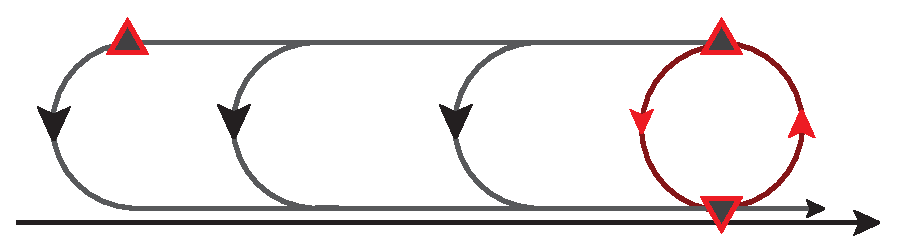
\includegraphics[scale=0.66]{StandardScheme.eps}};
    \node at (31mm,-15mm) [anchor=center] {\texttt{START}};
    \node at (31mm,14mm) [anchor=center] {\texttt{TURN\_END}};
    \node at (-35mm,14mm) [anchor=center] {\texttt{BACK\_END}};
  \end{tikzpicture}

  \caption{Стандартная схема задержки}
  \label{fig:StScheme}
\end{figure}


Формат описания стандартных схем:
\begin{center}
  \verb|NAME (START)(REPEAT) : START TURN_END BACK_END|
\end{center}
Здесь:
\begin{description}[topsep=-0.5\parsep,itemsep=-0.5\parsep]
  \item[\texttt{NAME}] --- название схемы, последовательность букв и цифр; 
  \item[\texttt{START}] --- имя начальной точки схемы, точки начала дуги обратного разворота (см. рис.~\ref{fig:StScheme}); эта же точка является первой из трех в списке точек, определяющих схему;
  \item[\texttt{TURN\_END}] --- точка конца дуги обратного разворота  (см. рис.~\ref{fig:StScheme});
  \item[\texttt{BACK\_END}] --- точка, ограничивающая отрезок обратного движения ВС  (см. рис.~\ref{fig:StScheme});
  \item[\texttt{REPEAT}] --- натуральное число, означающее максимальное количество проходов одного ВС по схеме.
\end{description}

\medskip

По итогам тестирования программы на реальных трассах, выяснились некоторые типовые ситуации. После чего в процедуру чтения был встроен некоторый <<синтаксический сахар>>:
\begin{enumerate}[topsep=-0.5\parsep,itemsep=-0.5\parsep]
  \item в описании стандартной схемы можно опустить часть <<\texttt{(START)}>>; начальная точка будет взята из списка;
  \item если линейная схема состоит только из двух точек 

  \centerline{<<\texttt{NAME (START)(FINISH) : START FINISH}>>,} 

  то две точки после двоеточия можно опустить: <<\texttt{NAME (START)(FINISH) : }>>.
\end{enumerate}

\medskip

Примеры:
\begin{itemize}
  \item \texttt{NameA (DIPOP)(EE500 KOLOS): Str(KOLOS) DIPOP EE500 /Str}
  \item {\ttfamily NameB (KOLOS)(BEKAR) : KOLOS VALET Str(RODEL) EE020 EE021 EE022 EE023

  EE024 EE025 /Str RODEL BEKAR}

  \item \texttt{NameС (RODEL)(RW25R): RODEL BEKAR KVOTA EE252 EE253 RW25R}
  \item \texttt{NameStScheme (GALEB)(5): GALEB N1 N2}
\end{itemize}


\subsubsection{Структуры хранения}
\label{sec:SchemeStructures}

Для хранения линейных схем и схем со спрямлением используется следующая структура
\begin{verbatim}
struct Scheme {
  string name;
  int start;
  vector<int> path;
  vector<int> end;
  vector<int> straighteningFrom;
  vector<int> straighteningWhere;
}; 
\end{verbatim}

Поле \texttt{name} хранит имя схемы, по которому она будет упоминаться при построении потоков, поле \texttt{start}~--- индекс начальной точки. 

Массив \texttt{path} хранит индексы всех точек линейной части схемы. В случае схемы со спрямлением это точки идущие до токена \texttt{Str}, между токенами \texttt{Str} и \texttt{/Str}, и после токена \texttt{/Str}.

Массив \texttt{end} хранит индексы всех точек, считающимися концевым для данной схемы.

Массив \texttt{straighteningFrom} хранит индексы точек, описывающих участок с которого можно спрямляться. Соответственно, массив \texttt{straighteningFrom} хранит индексы точек, на которые можно спрямляться.

\medskip

Для хранения стандартных схем предназначена структура
\begin{verbatim}
struct StandardScheme {
  string name;
  int start;
  int seсond; 
  int third; 
  int repeat;
  Time Tmin = Time::createTsec(0);
  Time Tmax = Time::createTsec(0);
};
\end{verbatim}

Поле \texttt{name} хранит имя схемы. Поля \texttt{start}, \texttt{second} и \texttt{third} хранят индексы точек \texttt{START}, \texttt{TURN\_END} и \texttt{BACK\_END}, соответственно (см.~рис.~\ref{fig:StScheme}). Поле \texttt{repeat} хранит максимальное число проходов по схеме. 

Как будет сказано ниже, обработка стандартных схем происходит специальным образом, поэтому поля \texttt{Tmin} и \texttt{Tmax} хранят минимальное и максимальное время прохождения по схеме.

\medskip

В файле данных схема так же, как и точки, идентифицируются своими именами. Однако при работе с ними важной является их не идентификация по имени, как это происходит с точками, а идентификация по первой точке~--- для соединения схем в поток. Для хранения этой информации предназначен словарь

\centerline{\texttt{map<int, int> startPointIDtoStSchemeID;},}

\noindent
который заполняется при чтении схем.


\subsubsection{Процедура чтения}
\label{sec:ReadingSchemes}

Текстовое представление схем является самым сложным среди всех объектов, используемых в программе. Сложность обуславливается переменным размером данных~--- разные схемы состоят из разного количества точек, а также опциональностью отдельных элементов представления. Линейная схема и схема со спрямлением разнятся отсутствие или наличием участка спрямления. В схеме со спрямлением могут быть, а могут отсутствовать линейные участки предшествующие и последующие участку спрямления. 

Были рассмотрены три возможности организации чтения этих сильно варьирующихся данных:
\begin{enumerate}[topsep=-0.5\parsep,itemsep=-0.5\parsep]
  \item ручной разбор строк;
  \item использование библиотеки реализации грамматик;
  \item использование регулярных выражений.
\end{enumerate}

Первый и второй подходы показались чрезмерно трудоемкими. Первый~--- из-за весьма значительного объема кода, который следует написать для разбора всех возможных вариантов входных данных. Второй~--- из-за высокого порога входа, из-за значительного объема материала, необходимого для изучения, чтобы использовать этот инструмент.

Поэтому в текущей версии программы для разбора строк с информацией о схемах используются регулярные выражение.

\medskip

\noindent
\textbf{Чтение линейных схем и схем со спрямлением.}

Для разбора строки с информацией о линейной схеме и схеме со спрямлением используется следующее регулярное выражение:
\begin{verbatim}
    (\w+)\s*
    (?:\((\w+)\))?\s*
    \(([\w\s]*|\d+)\)\s*
    :
    (?:
        \s*([\w\s]*)\s+
        (?:Str
            \(([\w\s]+)\)\s*
            ([\w\s]+)
        \/Str)?\s*
        ([\w\s]*)?
    )?
\end{verbatim}

Первая группа захвата --- это имя схемы. Представляет из себя любой набор букв и цифр.

Вторая группа --- это имя точки, с которой начинается схема.

Третья --- это список имен конечных точек схемы.

Далее после двоеточия следует основное тело схемы. 

Четвертая группа — это точки схемы, предшествующие спрямлению. Если оно отсутствует, то эта группа представляет из себя путь. Однако, в связи с тем, что после этой группы обязательно должен быть хотя бы один пробел, и если после последней точки схемы пробела не будет, то эта точка не попадёт в эту группу захвата. Её нужно искать в седьмой группе.

Пятая группа --- это точки, на которые можно спрямляться с точек из шестой группы. Если спрямление в схеме отсутствует, то эти группы пустые. 

Седьмая группа --- это точки, идущие после спрямления. Или, если нет спрямления в схеме и нет пробела после последней точки, тогда тут находится та самая последняя точка.

Также для удобства записи схем состоящих из двух точек, было введено упрощение записи. Можно вводить только имя схемы, точку начала, точку конца и двоеточие. Что регулируется большой не захватывающей скобкой после двоеточия с вопросительным знаком на окончании.

Если спрямление присутствует, то путь состоит из четвёртой, шестой и седьмой групп захвата.

\medskip

\noindent
\textit{Заполнение структуры}. 

В общем случае первая группа сразу же присваивается в первое поле структуры. Второе поле --- это результат отображения Имя точки $\mapsto$ идентификатор точки, где в качестве имени выступает вторая группа захвата.

Далее необходимо заполнить массив конечных точек. Для этого используется вспомогательная функция, которая получает строку на вход и массив, который требуется заполнить. Строка читается поэлементно, и с помощью отображения Имя точки $\mapsto$ идентификатор точки заполняет данный массив. В случае, если точки не оказалось среди \textit{checkPoints}, тогда выдаётся ошибка и программа заканчивает свою работу с предупреждением о том, что в такой-то строке такая-та точка не найдена среди контрольных точек.

Затем абсолютно аналогично заполняются поля пять и шесть. Теперь необходимо собрать путь схемы. Для этого используя ту же вспомогательную функцию с четвёртой группой и полем путь, мы собираем точки до спрямления. Затем записываем в путь все элементы из поля пять, и, наконец, используя вспомогательную функцию с седьмой группой и полем путь, мы собираем точки после спрямления.

Если четвёртая и пятая группы пустые, то это означает, что мы имеем дело со схемой, состоящей из двух точек. В этом случае, имя и точка начала схемы заполняются как в общем случае, но также нам известно, что массив конечных точек состоит из одного элемента, поэтому мы можем его сразу же записывать в массив конечных точек. И тогда путь, также легко определяется, как точка начала схемы плюс первый, он же и единственный, элемент массива конечных точек.

\medskip

\noindent
\textbf{Чтение стандартных схем.}

Для разбора данных о стандартной схеме используется следующее регулярное выражение:
\begin{verbatim}
    (\w+)\s*
    (?:\((\w+)\))?\s*
    \(([\w\s]*|\d+)\)\s* 
    :
    (?:
        \s*([\w\s]*)\s+
        (?:Str
          \(([\w\s]+)\)\s*
          ([\w\s]+)
        \/Str)?\s*
        ([\w\s]*)?
    )?
\end{verbatim}

Первая группа захвата --- это имя стандартной схемы. Так как начало и конец совпадают, то вторая группа захвата это второе поле структуры. Третья группа --- это количество повторений схемы.

В стандартной схеме нет спрямлений, поэтому пятая и шестая группы всегда пустые. Четвёртая и седьмая вместе дают все три точки. Поэтому с помощью вспомогательной функции из обычных схем, заполняем временный массив \textit{path}, аналогичный одноименному полю из обычных схем. И, затем, заполняем второе, третье и четвёртые поля структуры стандартной схемы как --- первый, второй и третий элемент массива \textit{path}. Если же длина этого массива получилась больше трёх, то программа завершает работу и выдаёт ошибку.

Далее заполняется отображение идентификатор точки начала стандартной схемы $\mapsto$ идентификатор стандартной схемы.


%---------------------------------------------------------------------------------

\subsection{Данные о потоках}
\label{sec:flows}

Это самый простой файл.

В первой строке хранится количество потоков. Следующие строки хранят информацию о потоках в виде
\begin{center}
  ИМЯ\_ПОТОКА ИМЯ\_ПЕРВОЙ\_ТОЧКИ
\end{center}

Пример:
2\\
Flow1 DIPOP\\
Flow2 AKERA

\medskip

Однако несмотря на простоту входных данных, структура хранения данных по потоку достаточно содержательна:
\begin{verbatim}
  string name;
  int start_point;
  map<int, vector<int>> graph_of_descendants;
  map<int, vector<int>> graph_of_ancestors;
  vector<int> keys;
  map<int, vector<pair<Time, Time>>> times;
\end{verbatim}
Поле \texttt{name} --- имя потока, \texttt{start\_point}~--- индекс начальной точки потока. Эти поля заполняются непосредственно при чтении из файла.

Остальные поля хранят информацию об устройстве потока и вычисляются после чтения потока. Поля \texttt{graph\_of\_descendants} и \texttt{graph\_of\_ancestors} хранят информацию о связи точек в графе потока (соответственно, индексы потомков и предков каждой точки, входящей в поток и задаваемой своим индексом). 

Поле \texttt{keys} вспомогательное поле, заполняемое после топологической сортировки графа потока (см.~раздел~\ref{sec:TopSort}). Содержит набор индексов точек потока в порядке топологической сортировки. Нужно для обхода и обработки контрольных точек потока в порядке, гарантирующем обработку всех предков точки до обработки ее самой.

Поле \texttt{times} хранит результат работы программы: множество возможных моментов прибытия ВС в контрольную точку, индекс которой является ключом в словаре. Множество задается как список (\texttt{vector}) непересекающихся интервалов времени (структура \texttt{pair<Time, Time>}), упорядоченных по возрастанию левых концов.


\subsection{Данные по всей зоне}

Как видно из предыдущей части текста, данные, описывающие структуру воздушных трасс, весьма многочисленны и разнообразны. Поэтому они собраны в объект структуры типа
\begin{verbatim}
struct Zone {
  vector<CheckPoint> checkPoints;
  vector<Scheme> schemes;
  vector<StandardScheme> standardSchemes;
  vector<Flow> flows;
  vector<vector<int>> graph_of_descendants;
};
\end{verbatim}

Первые четыре поля~--- это массивы данных по контрольным точкам в зоне; схемам, линейным/со спрямлением и стандартным; Поле \texttt{graph\_of\_descendants} представляет собой полное описание графа точек во всей зоне. Из него черпаются данные для графов каждого из потоков (см.~раздел~\ref{sec:flows}).

В целом, данные программы это три глобальных объекта:
\begin{itemize}[topsep=-0.5\parsep,itemsep=-0.5\parsep]
  \item объект типа \texttt{Zone}, хранящий информацию о трассах зоны;
  \item объект \texttt{pointNameToID}, хранящий сопоставление имен контрольных точек и их индексов в массиве \texttt{checkPoints} (см.~раздел~\ref{sec:PointStructures});
  \item объект \texttt{startPointIDtoStSchemeID}, хранящий сопоставление имен схем и индексов их начальных точек в массиве \texttt{checkPoints} (см.~раздел~\ref{sec:SchemeStructures}).
\end{itemize}

\section{Работа программы}

\subsection{Чтение данных}

Чтение данных, в целом, представляет собой поочередное чтение данных из файлов и заполнение этих трёх объектов. Сначала считываются точки, потом схемы, затем потоки. Каждая читается с помощью регулярных выражений в соответствии с форматом.

Основная идея одинакова для всех трёх файлов. Процедура, соответствующая файлу, получает на вход путь к нему и массив структур, который требуется заполнить. Далее объявляется счётчик, который отвечает за движение по массиву. Затем делается попытка открыть файл. В случае успеха выводится сообщение об открытии файла, иначе выводится сообщение об ошибке, и программа останавливает свою работу. Если файл был открыт, то первым делом происходит считывание длины массива и проверка на не отрицательность этого числа. В случае, если полученная длина массива не положительна, то происходит остановка программы. Иначе длина массива становится равной полученному числу. Далее объявляется регулярное выражение для работы с данными из файла. 

Начинается основной цикл, в котором происходит заполнение массива. Файл читается построчно и построчно обрабатывается регулярным выражением до тех пор, пока не закончится файл. Первым делом делается проверка на успешность сопоставления регулярного выражения и строки. В случае неуспеха выводится сообщение о несоответствии формату. Также проверяется уникальность имён входных данных. Далее делается проверка на возможность доступа к текущей координате массива. В случае невозможности осуществить это программа заканчивает работу и предупреждает о нехватке выделенного места под элементы массива. Затем идёт заполнение, подробности которого можно найти ниже. И, наконец, после успешного наполнения массива, делается проверка и правка, чтобы действительная длина массива совпадала с декларируемой, если это не так, то производится коррекция, после чего файл закрывается.

\subsection{Предобработка считанных данных}

После того, как все данные считаны производится их предварительная обработка.

Сначала заполняем поля времён у стандартных схем. Минимальное время --- пролёт по окружности с максимальной скоростью, а максимальное --- пролёт по всей схеме с минимальной скоростью.

Обозначим точки стандартной схемы $\nu_0 = (x_0, y_0, z_0),~ \nu_1 = (x_1, y_1, z_1),~ \nu_2 = (x_2, y_2, z_2)$
Вычислим радиус поворота как половину от расстояния между $\nu_0$ и $\nu_1$:
$$
  R = \frac{1}{2} \ast \sqrt{(x_1 - x_0)^2 + (y_1 - y_0)^2 + (z_1 - z_0)^2}
$$
Длину плеча находится как расстояние между $\nu_1$ и $\nu_2$:
$$
  S = \sqrt{(x_2 - x_1)^2 + (y_2 - y_1)^2 + (z_2 - z_1)^2}
$$
Тогда минимальное и максимальное времена выражаются следующим образом:
$$
  T_{min} = \frac{2 \pi R}{v_{max}}, \qquad 
    T_{max} = \frac{2(S + \pi R)}{v_{min}},
$$
где $v_{max}$ и $v_{min}$ --- это максимально и минимально возможные скорости первой точки схемы.

Граф зоны будем строить списками следующих. То есть соединяем ребрами данную вершину, со всеми вершинами, которые имеют связь с данной. Делать это будем следующим образом: идём по массиву линейных схем/схем со спрямлением, обрабатывая каждую схему в отдельности. На данном этапе нас интересует поле \textit{path}. Так как в нём лежат вершины в порядке прохождения самолётом схемы, то мы будем соединять текущую точку со следующей. Далее нужно соединить вершины, с которых возможно спрямление со всеми вершинами на которые это спрямление доступно. После чего переходить к другой схеме. Но есть нюанс. Если из предпоследней точки схемы можно спрямиться на конечную, то возникает проблема с добавлением этого ребра дважды --- первый раз как элемент пути, второй как элемент спрямления. Это необходимо учесть. 


\subsection{Построение графов потоков}

Теперь построим граф потока, как подграф графа зоны, также списками потомков. Для этого воспользуемся поиском в глубину. Заведём стек, на который будем складывать не посещённые вершины и массив меток, в котором будем отмечать посещённые вершины. Будем работать до тех пор, пока стек не опустеет. Сначала складываем на него точку начала потока. Используя граф зоны, соединяем эту точку со всеми сыновьями, и если сын ещё не посещён, то добавляем его на стек и ставим метку, что его посетили. В результате получим граф потока. После собираем граф потока, заданный списками предшественников, путём перебора графа, построенного списками потомков.

%---------------------------------------------------------------------------------


\subsection{Топологическая сортировка графов потоков}
\label{sec:TopSort}

К полученным ориентированным графам потоков применяется топологическая сортировка для получения порядка обработки точек потока, гарантирующего, что никакая точка не будет обработана ранее какого-либо из своих предков. Для хранения полученного порядка вершин используется поле \textit{keys} записи потока. Это массив, хранящий идентификатор в топологически отсортированном порядке $\mapsto$ идентификатор в исходном порядке. Сортировка проводится методом полустепеней захода. Заведём переменную \textit{number}, которая будет помогать отсортировывать вершины, инициализируем её нулём. Сначала сделаем размер массива ключей равным количеству вершин в потоке. Затем инициализируем отображение Точка $\mapsto$ полу степень захода следующим образом всем вершинам сопоставляется ноль. Заполняем его так: идя по спискам потомков, увеличиваем значение на единицу за каждого предка у вершины. Заводим стек и складываем на него все вершины с нулевой полустепенью захода. Пока стек не пуст, берём вершину со стека и на место number в массиве записываем идентификатор вершины. Увеличиваем \textit{number} на единицу. И для всех потомков данной вершины уменьшаем на единицу полустепень захода, и, если она стала равна нулю --- кладём этого потомка на стек. В результате получаем нужный массив.


%---------------------------------------------------------------------------------


\subsection{Вспомогательная процедура объединения двух множеств моментов прибытия}

На вход дается массив пар действительных чисел, упорядоченных по возрастанию первых элементов и задающих набор отрезков. Отрезки могут вкладываться и/или пересекаться. Необходимо конвертировать этот набор в эквивалентный набор непересекающихся отрезков, произведя объединение пересекающихся поднаборов. Будем делать с помощью отображения число $\mapsto$ действие. Для корректного сравнения действительных чисел реализованы два компаратора для проверки что одно число больше или меньше другого с точностью $\epsilon$, заданной в классе времени (по умолчанию $\epsilon = 10^{-4}$). Сначала проверим, что пары заданы корректно, то есть первый элемент меньше либо равен второго, иначе программа завершает работу и выдаёт сообщение об ошибке. Затем инициализируем нулевыми значениями отображение и заполняем его, если элемент стоит на первом месте в паре, тогда его значение увеличиваем на единицу, если на втором, то уменьшаем на единицу. Очистим массив времён. Заведём переменную, в которой будем считать сумму, инициализировав нулём. Вместе с тем, запомним первый элемент и назовём его начальным. Идём до конца ассоциативного массива, суммируя с накоплением значения отображения. Если в какой-то момент сумма стала равна нулю, то добавляем пару, состоящую из первого элемента, который мы запомнили, и текущего элемента. Проверяем, если мы не дошли до конца ассоциативного массива, то следующий элемент объявляем начальным и продолжаем цикл. В результате мы объединили вложенные и пересекающиеся интервалы, остались лишь непересекающиеся.


%---------------------------------------------------------------------------------


\subsubsection{Вычисление возможных времен прибытия ВС в контрольные точки}

Будем рассчитывать время для каждого потока по отдельности.

Так как поток топологически отсортирован, мы будем двигаться по возрастанию идентификатора вершин до тех пор, пока не дойдём до вершины с максимальным индексом, рассчитывая возможное время прибытия в следующие точки из данной. Сразу же выполним объединение времён, так как с прошлого шага мы получили набор интервалов, не обязательно не пересекающихся. 

Требует отдельного рассмотрения стандартная схема. Если в данная точка является началом стандартной схемы, у которой остались повторения, то нужно к текущим временным интервалам данной точки добавить интервалы, полученные прибавлением $T_{min}$ и $T_{max}$ из полей стандартной схемы к каждому из имеющихся интервалов данной точки, и уменьшить количество повторений этой стандартной схемы на единицу. 

Если же стандартной схемы нет или она исчерпала себя, то тогда для всех потомков время вычисляется как равнопеременное:
$$
  T_{min} = \frac{2S}{v_{max}^0 + v_{max}^1}
$$
где $v_{max}^0$ --- это максимально допустимая скорость на текущей контрольной точке, а $v_{max}^1$ --- это максимально допустимая скорость на данном потомке текущей контрольной точке
$$
  T_{max} = \frac{2S}{v_{min}^0 + v_{min}^1}
$$
где $v_{min}^0$ --- это минимально допустимая скорость на текущей контрольной точке, а $v_{min}^1$ --- это минимально допустимая скорость на данном потомке текущей контрольной точке, а $S$ --- евклидово расстояние между точками:
$$
  S = \sqrt{(x_1 - x_0)^2 + (y_1 - y_0)^2 + (z_1 - z_0)^2}.
$$

После чего добавляем к каждому интервалу полученные $T_{min}$ и $T_{max}$, и этот новый интервал записываем в массив времён потомка. И увеличиваем счётчик на единицу. После выполнения цикла получаем набор временных интервалов для каждой точки из потока.

Выполняя данную процедуру для каждого из потоков, получим набор временных интервалов для каждой точки.


\newpage
%=======================================================================

\section{Примеры расчётов}

\subsection{Простейшие случаи}

Рассмотрим работу процедуры в простейших случаях на данном примере:

\begin{figure}[h]
  \begin{center}
      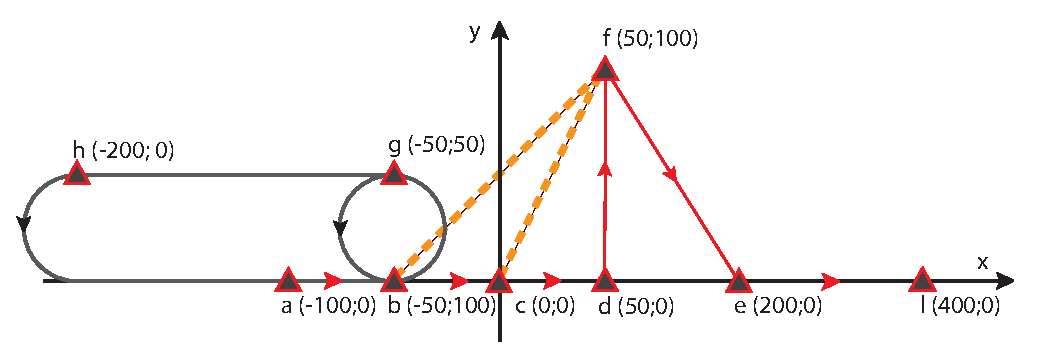
\includegraphics[width=0.95\textwidth]{Example.eps}
        \caption{Макетный пример}                                                                             
  \end{center}
\end{figure}

Пусть расстояние будет в метрах, а скорость в метрах в секунду.

\noindent Файл с данными точек:\\
9\\
a -100 0 0 5 10\\
b -50 0 0 5 10\\
c 0 0 0 5 10\\
d 50 0 0 5 10\\
e 200 0 0 4 6\\
f 50 100 0 4 8\\
g -50 50 0 5 10\\
h -200 50 0 5 10\\
r 400 0 0 2 5 LAND\\

\noindent Файл с данными схем:\\
3\\
1\\
Name1 (e)(r):\\
Name2 (a)(e): a Str(f) b c d /Str f e\\
NameSt1 (0): b g h\\

\noindent Файл с данными потоков:\\
3\\
Flow1 e\\
Flow2 a\\

\subsubsection{Движение по прямой}


Рассмотрим движение по прямой на примере первого потока:


$$
T_{min} = \frac{2S}{v_{max}^e + v_{max}^r} = \frac{2\cdot\sqrt{(400 - 200)^2}}{6 + 5} \approx 36.(36)\,\text{с}
$$

$$
T_{max} = \frac{2S}{v_{min}^e + v_{min}^r} = \frac{2\cdot\sqrt{(400 - 200)^2}}{4 + 2} \approx 66.(66)\,\text{с}
$$

И результат процедуры:

\noindent Flow1:\\
e $\rightarrow$ [0~с, 0~с]\\
r $\rightarrow$ [36.36~с, 66.67~с]


%---------------------------------------------------------------------------------

\subsubsection{Движение по вееру и прямым участкам}

Движение по вееру и прямым участкам рассмотрим на примере второго потока. Рассчитаем временной интервал для точки $f$:

\begin{multline}
T_{min} = \frac{2S_{a-b}}{v_{max}^b + v_{max}^a} + \frac{2S_{b-f}}{v_{max}^f + v_{max}^b}
= \frac{2\cdot\sqrt{(-50 + 100)^2}}{10 + 10} + \frac{2\cdot\sqrt{(50 + 50)^2 + (100-0)^2}}{8 + 10} \approx \\
 \approx 20.71348\,\text{с}
\end{multline}

\begin{multline}
T_{max} = T_{max}^{a-b} + T_{max}^{b-c} + T_{max}^{c-d} + T_{max}^{d-f} = 
 \frac{2S_{a-b}}{v_{min}^b + v_{min}^a} + \frac{2S_{b-c}}{v_{min}^c + v_{min}^b} +
 \frac{2S_{c-d}}{v_{min}^d + v_{min}^c} + \frac{2S_{d-f}}{v_{min}^f + v_{min}^d} = \\
 =\frac{2\cdot\sqrt{(-50 + 100)^2}}{5 + 5} + \frac{2\cdot\sqrt{(0 + 50)^2}}{5 + 5} +
 \frac{2\cdot\sqrt{(50 - 0)^2}}{5 + 5} + \frac{2\cdot\sqrt{(50 - 50)^2 + (100-0)^2}}{5 + 4} = \\
 = 10 + 10 + 10 + 22.(2) = 52.(2)\,\text{с}
\end{multline}

Результат процедуры:\\
Flow2:\\
a $\rightarrow$ [0~с, 0~с]\\
b $\rightarrow$ [5~с, 10~с]\\
c $\rightarrow$ [10~с, 20~с]\\
d $\rightarrow$ [15~с, 30~с]\\
f $\rightarrow$ [20.71~с, 52.22~с]\\
e $\rightarrow$ [46.47~с, 97.29~с]\\
r $\rightarrow$ [82.83~с, 163.96~с]\\


%---------------------------------------------------------------------------------

\subsubsection{Движение по вееру и прямым участкам со стандартной схемой}

Теперь изменим файл схем следующим образом --- добавим одно повторение к стандартной схеме:

\noindent 3\\
1\\
Name1 (e)(r):\\
Name2 (a)(e): a Str(f) b c d /Str f e\\
NameSt1 \underline{(1)}: b g h

И запустим поток с точки a:

\noindent 1\\
Flow1 a

Посчитаем время минимальной и максимальной задержки для этой стандартной схемы:

Вычислим радиус поворота, как половину от расстояния между b и g:

$$
 R = \frac{1}{2} \cdot \sqrt{(-50 + 50)^2 + (50 - 0)^2} = 25\,\text{м}
$$

Длину плеча найдём, как расстояние между h и g:

$$
S = \sqrt{(-200 + 50)^2 + (50 - 50)^2} = 150\,\text{м}
$$

$$
T_{min} = \frac{2 \pi R}{v_{max}^b} = \frac{2 \pi \cdot 25}{10} = 5\pi \approx 15.7\,\text{с}
$$

$$
T_{max} = \frac{2(S + \pi R)}{v_{min}^b} = \frac{2(150 + \pi \cdot 25)}{5} = 60 + 10\pi \approx 91.4\,\text{с}
$$

Результат процедуры:

\noindent Flow1:\\
a $\rightarrow$ [0~с, 0~с]\\
b $\rightarrow$ [5~с, 10~с] [20.71~с, 101.42~с]\\
c $\rightarrow$ [10~с, 20~с] [25.71~с, 111.42~с]\\
d $\rightarrow$ [15~с, 30~с] [30.71~с, 121.42~с]\\
f $\rightarrow$ [20.71~с, 143.64~с]\\
e $\rightarrow$ [46.47~с, 188.71~с]\\
r $\rightarrow$ [82.83~с, 255.37~с]\\


Как можно заметить, появился новый временной интервал, соответствующий проходу по стандартной схеме.

\newpage

%======================================================================


\subsection{Расчёты для аэропорта <<Кольцово>>}

Рассмотрим работу программы на примере аэропорта Кольцово.

Общий вид зоны Кольцово представлен на рис.~\ref{KoltsAll}. Вид внутренней зоны представлен на рис.~ \ref{KoltsLand}

\begin{figure}[h]
  \begin{center}
      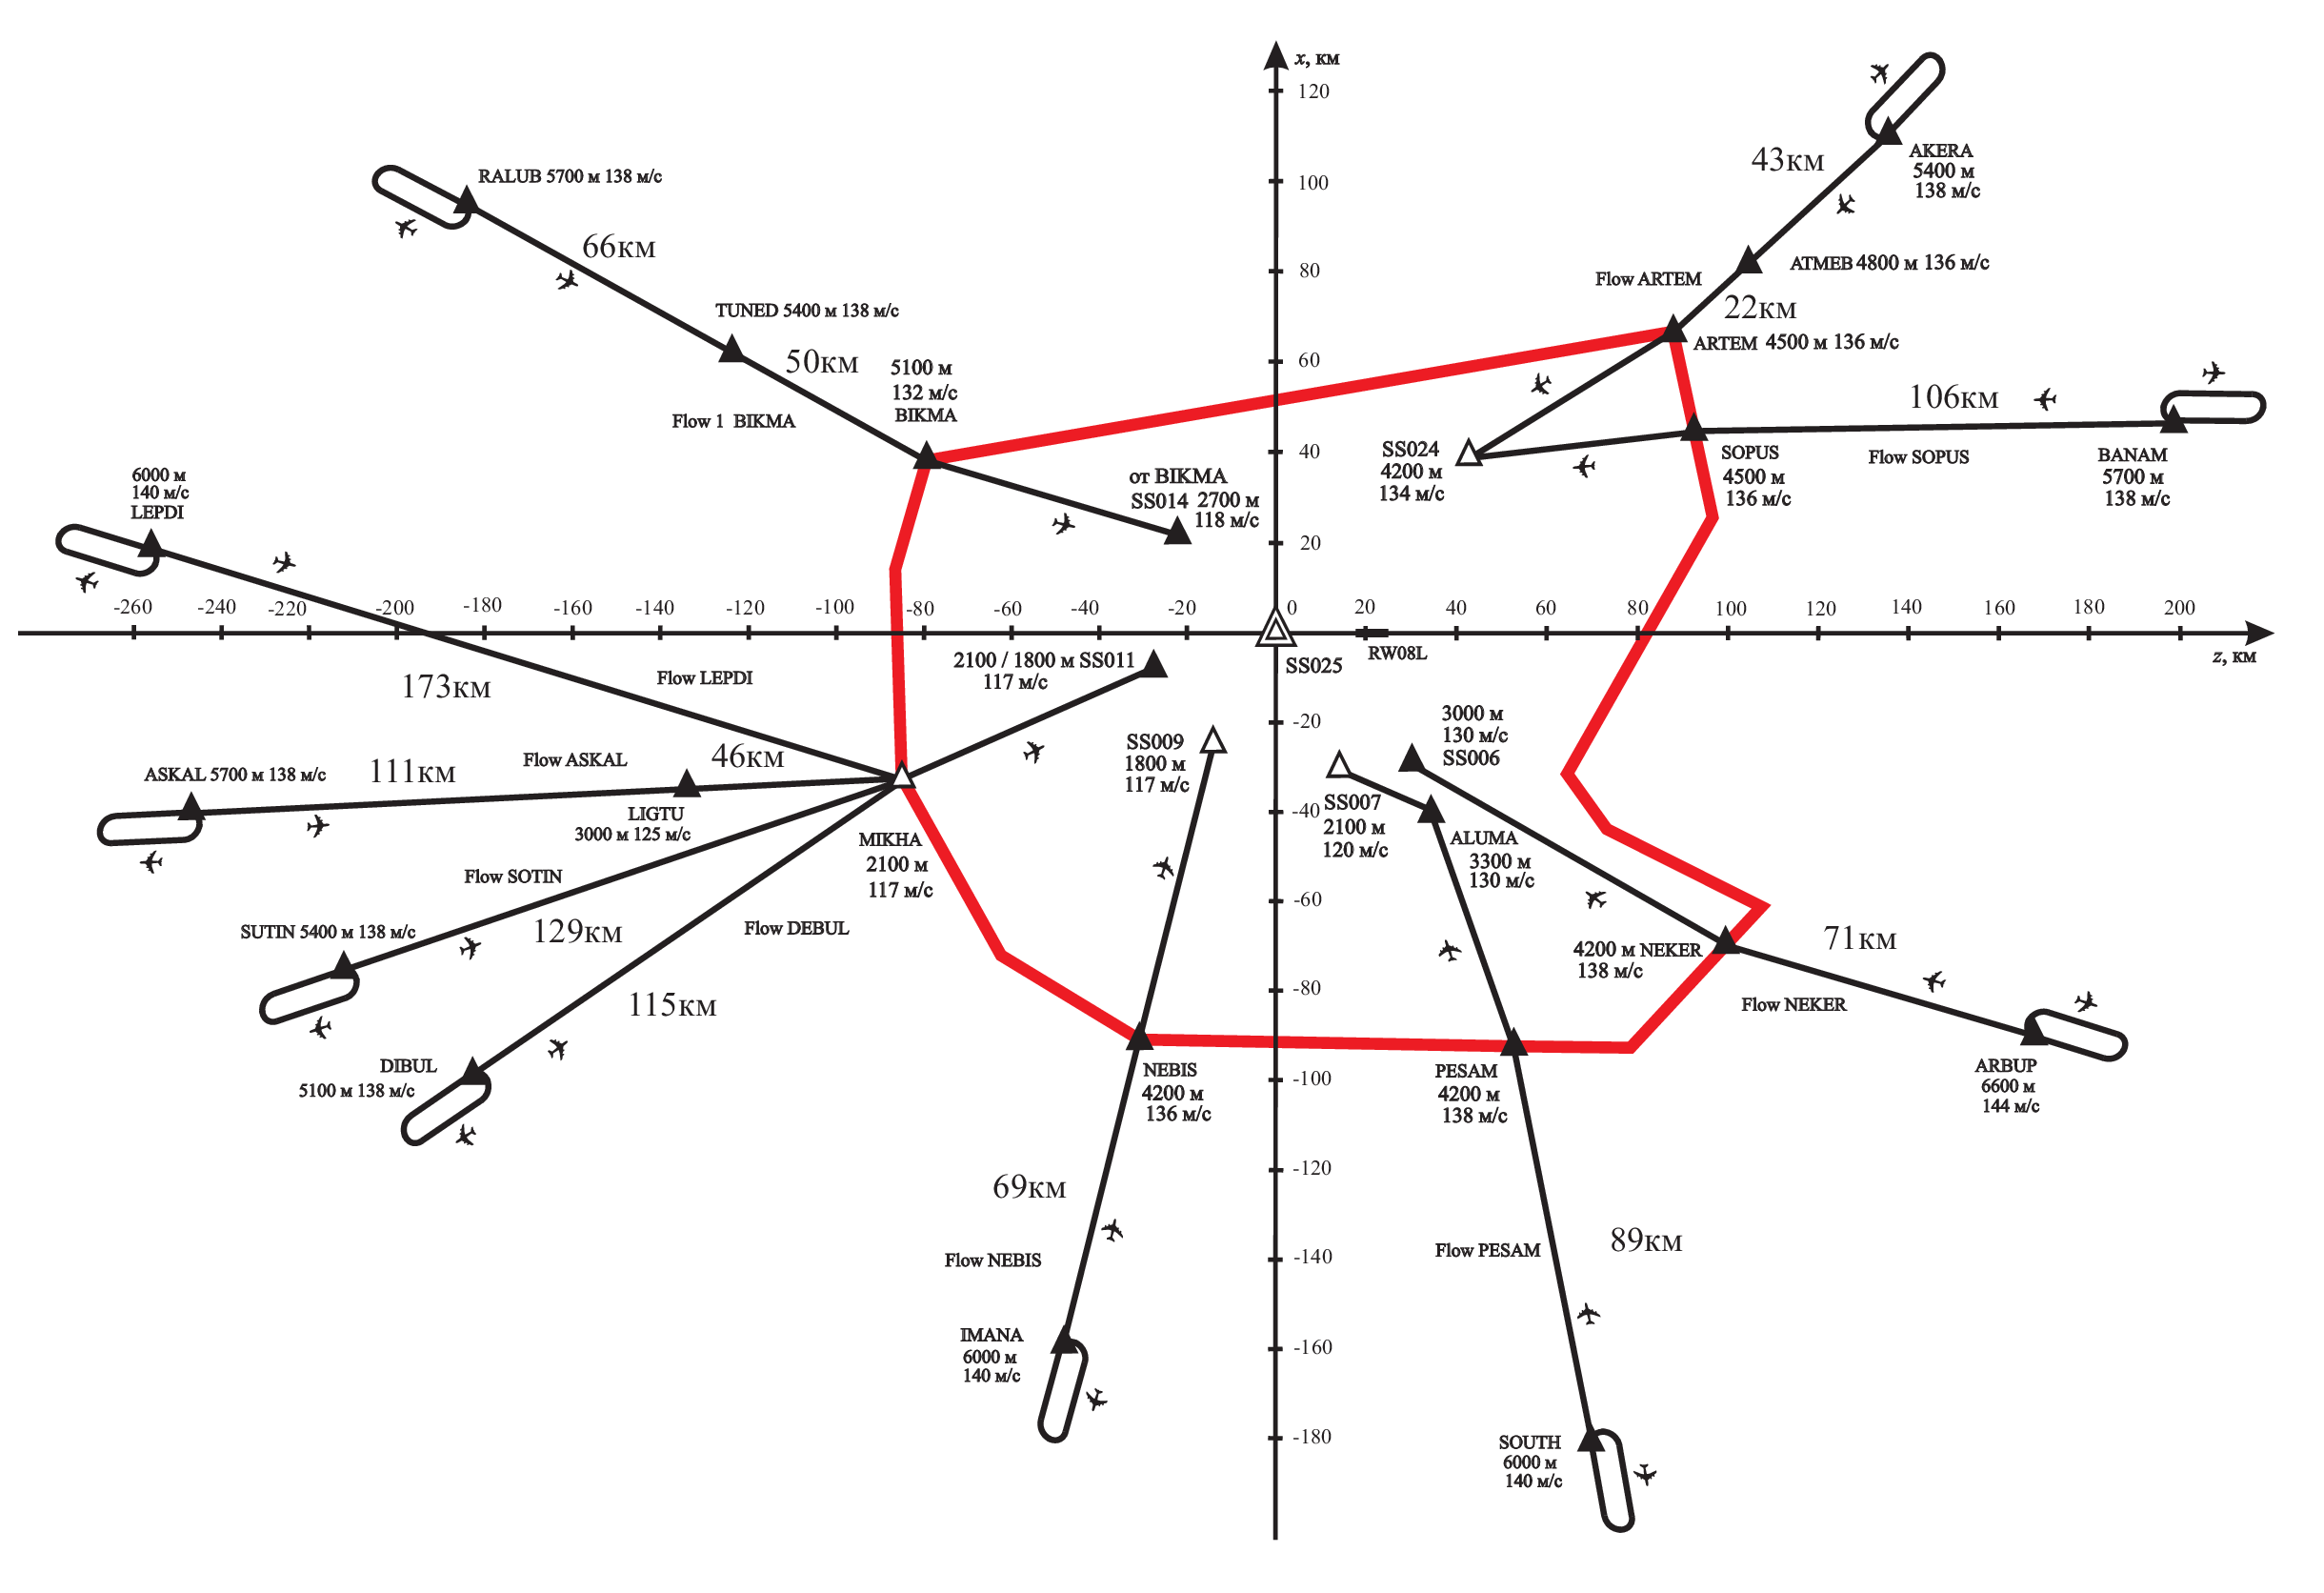
\includegraphics[scale=0.25]{Koltsovo01.png}
        \caption{Общий вид зоны Кольцово}                                                                             
    \label{KoltsAll}
  \end{center}
\end{figure}

\begin{figure}[h]
  \begin{center}
      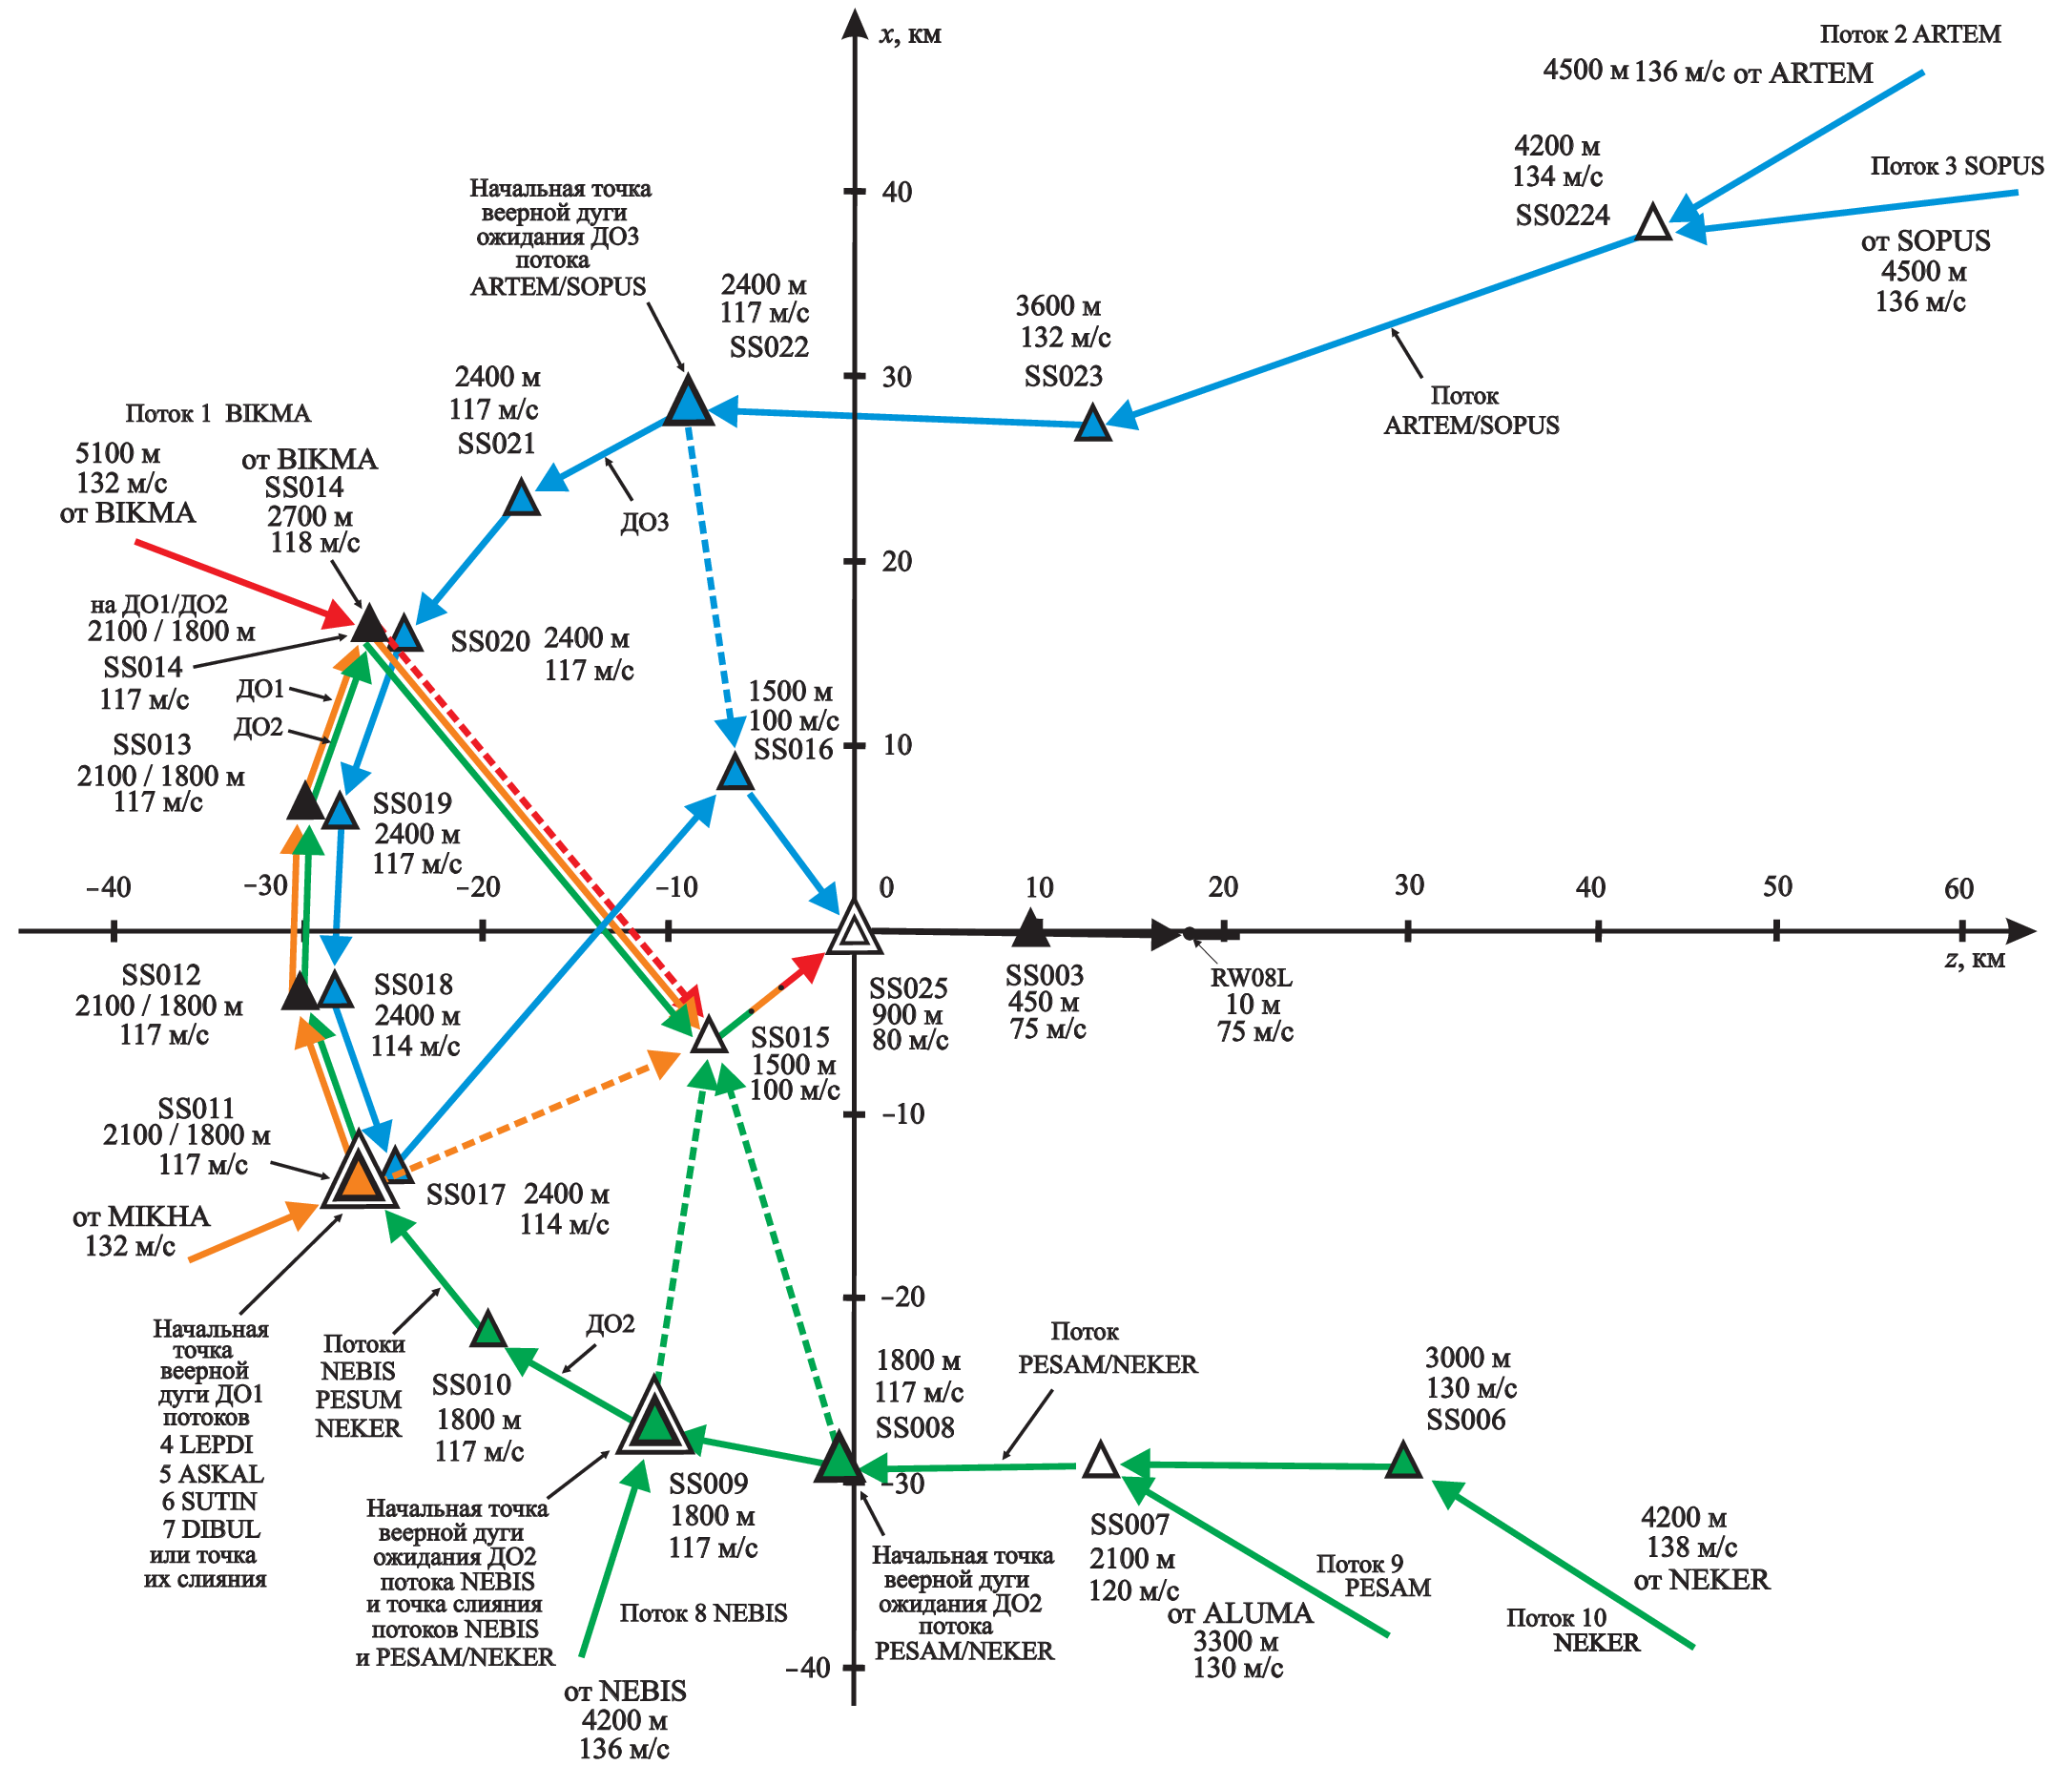
\includegraphics[scale=0.25]{Koltsovo02.png}
        \caption{Прибывающие потоки и веерные схемы их слияния.}                                                                             
    \label{KoltsLand} 
  \end{center}
\end{figure}

Рассмотрим поток BIKMA начинающийся в точке RALUB.

Результаты работы процедуры для потока BIKMA с нулём повторений стандартной схемы:

\noindent Flow1BIKMA:\\
RALUB $\rightarrow$ [0~с, 0~с]\\
TUNED $\rightarrow$ [474.52~с, 548.67~с]\\
BIKMA $\rightarrow$ [818.27~с, 947.42~с]\\
SS014 $\rightarrow$ [1240.52~с, 1443.1~с]\\
SS015 $\rightarrow$ [1482.57~с, 1734.04~с]\\
SS025 $\rightarrow$ [1578.33~с, 1853.75~с]\\
SS003 $\rightarrow$ [1684.27~с, 1991.08~с]\\
RW08L $\rightarrow$ [1792.31~с, 2132.36~с]\\


Результаты работы процедуры для потока BIKMA c однократным повторением стандартной схемы:

\noindent Flow1BIKMA:\\
RALUB $\rightarrow$ [0~с, 0~с] [389.33~с, 992.17~с]\\
TUNED $\rightarrow$ [474.52~с, 548.67~с] [863.86~с, 1540.84~с]\\
BIKMA $\rightarrow$ [818.27~с, 947.42~с] [1207.61~с, 1939.58~с]\\
SS014 $\rightarrow$ [1240.52~с, 1443.1~с] [1629.85~с, 2435.26~с]\\
SS015 $\rightarrow$ [1482.57~с, 1734.04~с] [1871.9~с, 2726.21~с]\\
SS025 $\rightarrow$ [1578.33~с, 1853.75~с] [1967.66~с, 2845.91~с]\\
SS003 $\rightarrow$ [1684.27~с, 1991.08~с] [2073.6~с, 2983.24~с]\\
RW08L $\rightarrow$ [1792.31~с, 2132.36~с] [2181.64~с, 3124.52~с]\\


Рассмотрим поток NEKER начинающийся в точке ARBUP.

Результаты работы процедуры для потока NEKER с нулём повторений стандартной схемы:

\noindent Flow10NEKER:\\
ARBUP $\rightarrow$ [0~с, 0~с]\\
NEKER $\rightarrow$ [463.24~с, 533.96~с]\\
SS006 $\rightarrow$ [1015.68~с, 1175.5~с]\\
SS007 $\rightarrow$ [1140.14~с, 1321.61~с]\\
SS008 $\rightarrow$ [1249.54~с, 1451.18~с]\\
SS009 $\rightarrow$ [1331.5~с, 1548.45~с]\\
SS010 $\rightarrow$ [1413.66~с, 1645.98~с]\\
SS011a $\rightarrow$ [1496.1~с, 1743.82~с]\\
SS012a $\rightarrow$ [1578.68~с, 1841.84~с]\\
SS013a $\rightarrow$ [1661.3~с, 1939.91~с]\\
SS014aaa $\rightarrow$ [1743.95~с, 2038~с]\\
SS015 $\rightarrow$ [1455.79~с, 2330.19~с]\\
SS025 $\rightarrow$ [1551.56~с, 2449.89~с]\\
SS003 $\rightarrow$ [1657.5~с, 2587.22~с]\\
RW08L $\rightarrow$ [1765.54~с, 2728.5~с]\\



Результаты работы процедуры для потока NEKER с однократным повторением стандартной схемы в точке ARBUP:

\noindent Flow10NEKER:\\
ARBUP $\rightarrow$ [0~с, 0~с] [234.91~с, 925.33~с]\\
NEKER $\rightarrow$ [463.24~с, 533.96~с] [698.15~с, 1459.29~с]\\
SS006 $\rightarrow$ [1015.68~с, 1175.5~с] [1250.59~с, 2100.83~с]\\
SS007 $\rightarrow$ [1140.14~с, 1321.61~с] [1375.04~с, 2246.93~с]\\
SS008 $\rightarrow$ [1249.54~с, 1451.18~с] [1484.45~с, 2376.51~с]\\
SS009 $\rightarrow$ [1331.5~с, 1548.45~с] [1566.4~с, 2473.78~с]\\
SS010 $\rightarrow$ [1413.66~с, 1645.98~с] [1648.57~с, 2571.31~с]\\
SS011a $\rightarrow$ [1496.1~с, 2669.15~с]\\
SS012a $\rightarrow$ [1578.68~с, 2767.16~с]\\
SS013a $\rightarrow$ [1661.3~с, 2865.24~с]\\
SS014aaa $\rightarrow$ [1743.95~с, 2963.33~с]\\
SS015 $\rightarrow$ [1455.79~с, 3255.51~с]\\
SS025 $\rightarrow$ [1551.56~с, 3375.21~с]\\
SS003 $\rightarrow$ [1657.5~с, 3512.54~с]\\
RW08L $\rightarrow$ [1765.54~с, 3653.83~с]\\

\newpage
%=======================================================================

\section*{Заключение}
\addcontentsline{toc}{section}{Заключение}

В результате работы была решена поставленная задача о вычислении временных интервалов прибытия воздушного судна на контрольные точки. Процесс работы состоял в изучении задачи, выборе структур данных и алгоритмов. Реализации на языке C{}\verb!++! 14-го стандарта. В качестве примера была рассмотрена схема аэропорта <<Кольцово>> в городе Екатеринбурге.

\newpage
%=======================================================================


\begin{thebibliography}{9}
\addcontentsline{toc}{section}{Список литературы}

\bibitem{bib:grafAndMatr} Асанов, М. О. Дискретная математика: графы, матроиды, алгоритмы : учебное пособие / М. О. Асанов, В. А. Баранский, В. В. Расин. — 2-е изд. испр. и доп. СПб.: Лань, 2010. 368 с.

\bibitem{bib:Report:2019-07} Спиридонов А.А. Кумков С.С. Разработка и исследование формализаций задачи бесконфликтного слияния потоков воздушных судов. Отчёт о научно-экспериментальной работе «Алгоритмы и программное обеспечение обработки информации в АС УВД» по Договору №29-19У. (Этап~1). Том~3, июнь 2019 г., 25~стр.
 
\bibitem{bib:TblSherem} Проект структуры воздушного пространства МУДР. Стандартные маршруты прибытия на аэродром Шереметьево. Версия 03 ПСВП МУДР 8.5.1 (таблицы). ГосНИИГА, Москва, 2016.

\bibitem{bib:SchmSherem} Проект структуры воздушного пространства МУДР. Схемы захода на посадку на аэродром Шереметьево. Версия 03 ПСПВ. Стандартные маршруты прибытия на аэродром Шереметьево. Версия 04 ПСВП МУДР 8.5.1 (схемы). ГосНИИГА, Москва, 2016.

\bibitem{bib:EURO} Point Merge Integration of Arrival Flows Enabling Extensive RNAV Application and Continuous Descent. Operation Services and Environment Definition. Report, July 2010. Eurocontrol Experimental Center, Bretigny-sur-Orge.\\
\texttt{http://www.eurocontrol.int/eec/gallery/content/public..}

\bibitem{bib:NASA} Air Traffic Management Technology Demonstration--1 (ATD--1). NASA Report FS-2011-10-01-ARC. 2011.

\bibitem{bib:NITA} Пятко С.Г., Красов А.И. и др. Автоматизированные системы управления воздушным движением. Новые информационные технологии в авиации. СПб.: Изд. Политехника, 2004.

\bibitem{bib:KorolevEN} Королев Е. Н. Технологии работы диспетчеров управления воздушным движением. М.: Воздушный транспорт, 2000.

\bibitem{bib:GOST} ГОСТ 20058-80. Динамика летательных аппаратов в атмосфере. Термины, определения и обозначения. М.: Госстандарт, 1980.


\end{thebibliography}

\label{lastpage}

\end{document}
